\usepackage[utf8]{inputenc} %
\usepackage[T1]{fontenc}    %
\usepackage{url}            %
\usepackage{booktabs}       %
\usepackage{amsfonts}       %
\usepackage{nicefrac}       %
\usepackage{microtype}      %
\usepackage{xcolor}         %

\usepackage{tikz}
\usepackage[utf8]{inputenc} %
\usepackage[T1]{fontenc}    %
\usepackage{algorithm}
\usepackage{algorithmic}
\usepackage[algo2e]{algorithm2e} 
\usepackage{url}            %
\usepackage{booktabs}       %
\usepackage{amsfonts}       %
\usepackage{nicefrac}       %
\usepackage{microtype}      %
\usepackage{xcolor}         %
\usepackage{times}
\usepackage{epsfig}
\usepackage{graphicx}
\usepackage{amsmath}
\usepackage{numprint}
\usepackage{amssymb}
\usepackage{booktabs}
\usepackage{rotating}
\usepackage{makecell}
\usepackage{amssymb}%
\usepackage{pifont}%
\newcommand{\cmark}{\ding{51}}%
\newcommand{\xmark}{\ding{55}}%
\newcommand{\imgsunl}{62.2}%
\newcommand{\imgfunl}{76.7}%
\newcommand{\imgsl}{44.8}%
\newcommand{\imgfl}{72.8}%
\newcommand{\sparsemat}{\ensuremath{\gls{WeightMatrix}^{\mathrm{sparse}}}}
\newcommand{\sparsematn}[1]{\ensuremath{\gls{WeightMatrix}_#1^{\mathrm{sparse}}}}
\newcommand{\psoln}[1]{\ensuremath{(\gls{WeightMatrix}_#1^{\mathrm{sparse}},\gls{bias}_#1)}}
\newcommand{\fullheader}{&\multicolumn{5}{c|}{CUB-2011}&\multicolumn{5}{c|}{FGVC-Aircraft}&\multicolumn{5}{c|}{NABirds}&\multicolumn{5}{c}{Stanford Cars}\\
 &\multicolumn{3}{c|}{$\gls{nReducedFeatures}=2048$}&\multicolumn{2}{c|}{$\gls{nReducedFeatures}=50$}& \multicolumn{3}{c|}{$\gls{nReducedFeatures}=2048$}&\multicolumn{2}{c|}{$\gls{nReducedFeatures}=50$} &
 \multicolumn{3}{c|}{$\gls{nReducedFeatures}=2048$} & \multicolumn{2}{c|}{$\gls{nReducedFeatures}=50$} &\multicolumn{3}{c|}{$\gls{nReducedFeatures}=2048$} & \multicolumn{2}{c}{$\gls{nReducedFeatures}=50$} \\
 \gls{customLoss} & Dense  & Sparse  & Finet. & Sparse  & Finet. & Dense  & Sparse  & Finet. & Sparse  & Finet. & Dense  & Sparse  & Finet. & Sparse  & Finet.  & Dense  & Sparse  & Finet. & Sparse  & Finet. \\\midrule}
\newcommand{\fullablheader}{\input{ablheader}}
\newcommand{\bbheader}{\input{backboneheader}}
\newcommand{\lossheader}{\input{Lossheader}}
\newcommand{\cLWheader}{\input{clWheader}}
\newcommand{\fgvcheader}{\gls{fgvcheader}}
\newcommand{\stanfordheader}{\gls{stanfordheader}}
\newcommand{\cubheader}{\gls{cubheader}}
\newcommand{\imgnetheader}{\gls{imgnetheader}}
\newcommand{\birdsheader}{\gls{birdsheader}}
\newcommand{\inpercent}{ in percent}
\newcommand{\imgbldStatement}{ for \resnet{} on \imgnetheader{} using the pretrained dense model.}
\usepackage{svg}
\usepackage{multirow}
\usepackage{smartdiagram}
\usepackage{tikz}
\usepackage{csquotes}
\usepackage{caption}
\usepackage{arydshln}
\usepackage{subcaption}
\captionsetup[subfigure]{%
  justification =justified,%
  format=hang}
\usetikzlibrary{shapes.geometric, arrows, fit}

\usepackage[acronym,nogroupskip]{glossaries}

\usepackage{hyperref}       %




\def\httilde{\mbox{\tt\raisebox{-.5ex}{\symbol{126}}}}

    
\newglossaryentry{customLoss}
{
name={\ensuremath{\mathcal{L}_{\mathrm{div}}}},
description={Custom Loss für unterschiedliche Features}
}
\newglossaryentry{cLW}
{
name={\ensuremath{\beta}},
description={Gewichtung für customLoss}
}
\newglossaryentry{elaWeight}
{
name={\ensuremath{\lambda}},
description={Gewichtung für elasticNet}
}
\newglossaryentry{elaW}
{
name={\ensuremath{\alpha}},
long = {\ensuremath{\alpha\in[0,1]}},
description={Gewichtung zwischen l1 und l2 für elasticNet}
}
\newglossaryentry{trainDataset}
{
name={\ensuremath{\boldsymbol{D}_t}},
first = {\ensuremath{\boldsymbol{D}_t\in \mathbb{R}^{\gls{nTrainImages}\times 3\times w\times h}}},
description={LokalisierungMaps mit Missingness}
}
\newglossaryentry{nFeatures}
{
name={\ensuremath{n_{f}}},
description={Anzahl der verwendeten Features}
}
\newglossaryentry{nReducedFeatures}
{
name={\ensuremath{\gls{nFeatures}^*}},
description={Anzahl der verwendeten Features im Sparse Decision Layer}
}
\newglossaryentry{outputVector}
{
name={\ensuremath{\boldsymbol{y}}},
long = {\ensuremath{\boldsymbol{y}\in \mathbb{R}^{\gls{nClasses}}}},
description={Finaler Ausgang des Netzes}
}
\newglossaryentry{features}
{
name={\ensuremath{\boldsymbol{f}}},
description={Aus Bild berechnete Features}
}
\newglossaryentry{LocalizationMaps}
{
name={\ensuremath{\boldsymbol{L}}},
long = {\ensuremath{\boldsymbol{L}_p}\in \mathbb{R}^{\gls{nReducedFeatures}\times \frac{w}{p}\times \frac{h}{p}}},
description={LokalisierungMaps mit Missingness}
}
\newglossaryentry{featuresMapwidth}
{
name={\ensuremath{ w_M}},
description={Weite der FeatureMap}
}
\newglossaryentry{featuresMapheigth}
{
name={\ensuremath{ h_M}},
description={Weite der FeatureMap}
}
\newglossaryentry{featureMaps}
{
first ={\ensuremath{\boldsymbol{M} \in \mathbb{R}^{\gls{nFeatures} \times \gls{featuresMapwidth}\times \gls{featuresMapheigth}}}},
name={\ensuremath{m}},
plural={\ensuremath{\boldsymbol{M}}},
description={Aus Bild berechnete Features}
}
\newglossaryentry{trainFeatures}
{
first ={\ensuremath{\boldsymbol{F}^{\mathrm{train}} \in \mathbb{R}^{\gls{nTrainImages} \times \gls{nFeatures}}}},
name={\ensuremath{\boldsymbol{F}^{\mathrm{train}}}},
description={Aus Bild berechnete Features}
}
\newglossaryentry{denseNet}
{
first = {DenseNet121~\citep{huang2017densely}},
name ={DenseNet121},
description={Final layer in the neural network}
}
\newglossaryentry{resNet}
{
first = {Resnet50~\citep{he2016deep}},
name ={Resnet50},
description={Final layer in the neural network}
}
\newglossaryentry{incv}
{
first = {Inception-v3~\citep{szegedy2016rethinking}},
name ={Inception-v3},
description={Final layer in the neural network}
}
\newglossaryentry{birdsheader}
{
first = {NABirds~\citep{7298658}},
name = {NABirds},
description={Final layer in the neural network}
}
\newglossaryentry{imgnetheader}
{
first = {ImageNet-1K~\citep{imagenet15russakovsky}},
long = {ImageNet-1K~\citep{imagenet15russakovsky}},
name={ImageNet-1K},
description={Final layer in the neural network}
}
\newglossaryentry{fgvcheader}
{
first = {FGVC-Aircraft~\citep{FGVCAircraft}},
name={FGVC-Aircraft},
description={Final layer in the neural network}
}
\newglossaryentry{stanfordheader}
{
first = {Stanford Cars~\citep{StanfordCars}},
name={Stanford Cars},
description={Final layer in the neural network}
}
\newglossaryentry{cubheader}
{
first = {CUB-2011~\citep{wah2011caltech}},
long = {CUB-2011~\citep{wah2011caltech}},
name={CUB-2011},
description={Final layer in the neural network}
}
\newglossaryentry{decisionLayer}
{
name={decision layer},
description={Final layer in the neural network}
}
\newglossaryentry{fittingLossTarget}
{
name={\ensuremath{\mathcal{L}_{\mathrm{target}}}},
description={Main goal of fitting}
}
\newglossaryentry{layerName}
{
name ={\textit{SLDD-Model}},
description={The proposed benchmark}
}
\newglossaryentry{denseLayer}
{
name={{dense high-dimensional \gls{decisionLayer}}},
description={The layer that results from training}
}
\newglossaryentry{correlationMatrix}
{
name={\ensuremath{\boldsymbol{Q}}},
first = {\ensuremath{\boldsymbol{Q}\in \mathbb{R}^{\gls{nFeatures}\times\gls{nFeatures}}}},
long = {\ensuremath{q}},
description={Correlation Matrix}
}
\newglossaryentry{featureVector}
{
name={\ensuremath{f}},
long={\ensuremath{\boldsymbol{f}}},
first ={\ensuremath{\boldsymbol{f} \in \mathbb{R}^{\gls{nFeatures}}}},
description={The features of the dense alyer}
}
\newglossaryentry{RedfeatureVector}
{
name={\ensuremath{\boldsymbol{f^*}}},
first ={\ensuremath{\boldsymbol{f^*} \in \mathbb{R}^{\gls{nReducedFeatures}}}},
description={The selected feature Vector}
}
\newglossaryentry{OnlyInteractionVector}
{
name={\ensuremath{\boldsymbol{P}}},
long={\ensuremath{\boldsymbol{P} \in \mathbb{R}^{ \gls{nInteractions}}}},
description={The Interaction Vector}
}
\newglossaryentry{InteractionVector}
{
name={\ensuremath{\boldsymbol{f^*_{\phi}}}},
first ={\ensuremath{\boldsymbol{f^*_{\phi}} \in \mathbb{R}^{\gls{nReducedFeatures} + \gls{nInteractions}}}},
description={The Extended Interaction Vector}
}
\newglossaryentry{nInteractions}
{
name={\ensuremath{n_I}},
description={number of interaction term}
}
\newglossaryentry{dnn}
{
name={\ensuremath{f_\theta(x})},
description={Deep neural network}
}

\newglossaryentry{bias}
{
name={\ensuremath{\boldsymbol{b}}},
long ={\ensuremath{\boldsymbol{b} \in \mathbb{R}^{\gls{nClasses}}}},
description={The bias in the decison layer}
}
\newglossaryentry{classifyFunc}
{
name={\ensuremath{C}},
description={The classifier on the featuers}
}
\newglossaryentry{WeightMatrix}
{
name={\ensuremath{\boldsymbol{W}}},
long = {\ensuremath{\boldsymbol{W}\in \mathbb{R}^{\gls{nClasses}\times \gls{nReducedFeatures} }}},
plural = {\ensuremath{w}},
description={The Weight matrix in the decision layer}
}

\newglossaryentry{nClasses}
{
name={n_c},
description={Number of Classes}
}
\newglossaryentry{nTrainImages}
{
name={\ensuremath{n_T}},
description={Number of Train Images}
}
\newglossaryentry{nWeights}
{
name={\ensuremath{n_w}},
description={Number of Entries != 0 in \gls{WeightMatrix}}
}
\newglossaryentry{nperClass}
{
name={\ensuremath{n_{wc}}},
description={Number of Entries != 0 in \gls{WeightMatrix} per Class}
}
\newglossaryentry{interpTrans}
{
name={\ensuremath{\phi}},
description={Interpretable Transformation}
}

\newglossaryentry{targetVector}
{
name={\ensuremath{\hat{\boldsymbol{y}}}},
description={Target Vector in Training}
}
\newglossaryentry{glmsaga}
{
first = {\mbox{\textit{glm-saga~\citep{wong2021leveraging}}}},
long = {\mbox{\textit{glm-saga~\citep{wong2021leveraging}}}},
name={\mbox{\textit{glm-saga}}},
description={Target Vector in Training}
}
\newglossaryentry{cbm}
{
name={\textit{CBM}},
first ={\textit{concept bottleneck models}~(\textit{CBM})~\citep{koh2020concept}},
long = {\textit{CBM}~\citep{koh2020concept}},
description={Target Vector in Training}
}
\newglossaryentry{ProtoPNet}
{
name={\textit{ProtoPNet}},
first ={\textit{ProtoPNet}~\citep{chen2019looks}},
description={Target Vector in Training}
}
\newglossaryentry{ProtoPShare}
{
name={\textit{ProtoPShare}},
first ={\textit{ProtoPShare}~\citep{rymarczyk2021protopshare}},
description={Target Vector in Training}
}
\newglossaryentry{ProtoPool}
{
name={\textit{ProtoPool}},
first ={\textit{ProtoPool}~\citep{rymarczyk2022interpretable}},
description={Target Vector in Training}
}
\newglossaryentry{ProtoTree}
{
name={\textit{Prototree}},
first ={\textit{ProtoTree}~\citep{nauta2021neural}},
description={Target Vector in Training}
}
\newglossaryentry{ImageSample}
{
name={\ensuremath{\boldsymbol{I}}},
first ={\ensuremath{\boldsymbol{I} \in \mathbb{R}^{3\times w\times h}}},
description={The classifier on the featuers}
}
\newcommand\tFs{5 }
\newcommand{\suppt}{}%
\newcommand{\incv}{\gls{incv}}
\newcommand{\resnet}{\gls{resNet}}
\newcommand{\densenet}{\gls{denseNet}}
\newcommand{\betaT}{ with varying~\gls{cLW} }
\newcommand{\attributeset}[1]{\ensuremath{\rho_{#1}}}
\newcommand{\classWeightsName}{\mbox{\textit{w/o Class-Specific}}}
\newcommand{\SoftmaxName}{\mbox{\textit{w/o Rescaling}}}
\newcommand\topFre{30\% }
\newcommand{\nth}[1]{#1\textsuperscript{th}}
\newcommand{\loc}[1]{\textrm{diversity@#1}}
\newcommand{\glm}{\gls{glmsaga}}
\newcommand{\tablefinisher}[1]{ dependent on #1}
\newcommand{\undlinstmt}{ Our used \gls{cLW} is underlined.}
\newcommand{\cbmauc}{\textit{CBM-AUC}~\citep{10.1109/access.2022.3167702}}
\newcommand{\pcbm}{\textit{PCBM}~\citep{yuksekgonul2022posthoc}}
\newcommand{\tableStatement}[1]{for number of features \mbox{$\gls{nReducedFeatures}=#1$} and features per class $\gls{nperClass}\leq5$}
\newcommand{\eg}{\textit{e}.\textit{g}. }
\newcommand{\KeptFeatures}{\ensuremath{N_{f^*}}}
\newcommand{\initFeatures}{\ensuremath{N_{f}}}
\newcommand{\wl}[1]{\ensuremath{\boldsymbol{w}_{#1}}}
\newcommand{\st}{s.\:t.}
\newcommand{\cmpLoss}{compared to other loss functions\bldStatement }
\newcommand{\arrowDown}{\ensuremath{\boldsymbol{\downarrow}}}
\newcommand{\ourstmt}{\textbf{Ours}}
\newcommand{\emptyStrichte}{ - & - & - & - & - &}
\newcommand{\fivetext}{five}
\newcommand{\fourtext}{four}
\newcommand{\arrowUp}{\ensuremath{\boldsymbol{\uparrow}}} %
\newcommand{\elude}{\textit{Elude}~\citep{elude} }
\newcommand{\comparison}[2]{
\begin{figure*}
     \begin{subfigure}[t]{.3\textwidth}
         \centering
          \includegraphics[width=\linewidth]{plots/ComparisonSparseDenseJpg/#2/Dense#2.png}
        \caption{Conventional Dense Model}
     \end{subfigure}
     \hfill
     \begin{subfigure}[t]{.3\textwidth}
         \centering
                 \includegraphics[width=\linewidth]{plots/ComparisonSparseDenseJpg/#2/Sparse#2.png}
            \caption{Sparse with $\gls{nReducedFeatures} = \gls{nFeatures}$}
     \end{subfigure}
     \hfill
     \begin{subfigure}[t]{.3\textwidth}
         \centering
         \includegraphics[width=\linewidth]{plots/ComparisonSparseDenseJpg/#2/Finetuned#2.png}
            \caption{Finetuned SLDD-Model}
     \end{subfigure}
     \caption{Feature maps of the top 5 features by magnitude for class #1 on example images. The used weights for the respective features are also displayed. }
        \label{app:fig:vizExamples#2}
\end{figure*}
}
\tikzstyle{process} = [rectangle, minimum width=1cm, minimum height=1cm, text centered, text width=1.8cm, draw=black]
\tikzstyle{decision} = [diamond, minimum width=1cm, minimum height=1cm, text centered, draw=black]
\tikzstyle{arrow} = [thick,->,>=stealth]


\title{Take 5: Interpretable Image Classification with a Handful of Features}%







\author{%
  Thomas Norrenbrock \quad Marco Rudolph \quad Bodo Rosenhahn \\
  Institute for Information Processing (tnt)\\
  L3S - Leibniz Universität Hannover, Germany \\
  \texttt{\{norrenbr, rudolph, rosenhahn\}@tnt.uni-hannover.de}} 




\begin{document}

\maketitle

\vspace{-5mm}
\begin{abstract}
\vspace{-3mm}
Deep Neural Networks use thousands of mostly incomprehensible features to identify a single class, a decision no human can follow.
We propose an interpretable sparse and low dimensional final decision layer in a deep neural network with measurable aspects of interpretability and demonstrate it on fine-grained image classification.
We argue that 
a human can only understand the decision of a machine learning model, if the features are interpretable and only very few of them are used for a single decision. For that matter, the final layer has to be sparse and - to make interpreting the features feasible - low dimensional. 
We call a model with a Sparse Low-Dimensional Decision \enquote{\gls{layerName}}.
We show that a \gls{layerName} is easier to interpret locally and globally than a \gls{denseLayer} while being able to maintain competitive accuracy. Additionally, we propose a loss function that improves a model's feature diversity and accuracy. 
Our more interpretable \gls{layerName} only uses 5 out of just 50 features per class,
while maintaining 97\,\% to 100\,\% of the accuracy on \fourtext{} common benchmark datasets compared to the baseline model with 2048 features.
\end{abstract}
\begin{figure}[bh!]
\begin{center}
   \includegraphics[width=0.5\linewidth]{plots/teaser_sldd.pdf}
\end{center}
   \caption{Local explanation by our \gls{layerName}: The two features used for the predicted class, emerged without additional supervision, are aligned with human interpretable attributes and localized (described in App.~\ref{app:featureViz}) adequately.}
   
\label{fig:Cover}
\end{figure}
\vspace{-10pt}
\section{Introduction}
\vspacehack{}
Understanding the decision of a deep learning model is becoming more and more important. Especially for safety-critical applications such as the medical domain or autonomous driving, it is often either legally~\citep{article} or by the practitioners required to be able to trust the decision and evaluate its reasoning~\citep{molnar2020interpretable}. 
Due to the high dimensionality of images, 
most previous work 
on interpretable models for computer vision
combines the deep features computed by a deep neural network with a method that is considered interpretable, such as a prototype based decision tree~\citep{nauta2021neural}.
While approaches for measuring the interpretability without humans exist for conventional machine learning algorithms~\citep{islam2020towards}, they are missing for methods including deep neural networks.
In this work, we propose a novel sparse and low-dimensional \gls{layerName} which offers measurable aspects of interpretability.
The key aspect is a heavily reduced number of features, out of which only very few are considered per class. Humans can only consider $7\pm 2$ aspects at once~\citep{miller1956magical} and could therefore follow a decision that uses that many features.
To be intelligible for all humans, we aim for an average of \tFs features per class. \\
 Having a reduced number of features makes it feasible to investigate every single feature and understand its meaning: We are able to align several of the learned features with human concepts post-hoc. The combination of reduced features and sparsity therefore increases both global \textit{How does the model behave?} and local interpretability \textit{Why did the model make this decision?}, demonstrated in Figure~\ref{fig:Cover}.\\
Our proposed method generates the \gls{layerName} by utilizing \glm{} to compute a sparse linear classifier for selected features, which we then finetune to the sparse structure.
We apply feature selection instead of a transformation to reduce the computational load and  preserve the original semantics of the features, which can improve interpretability~\citep{LDAForSelec}, especially if a more interpretable model like \textit{B-cos Networks}~\citep{bohle2022b} is used.
Additionally, we propose a novel loss function for more diverse features, which is especially relevant when one class depends on very few features, since using more redundant features limits the total information available for the decision.

Our main \textbf{contributions} are as follows:
\begin{itemize}

\item We present a pipeline that ensures a model with increased global and local interpretability which identifies a single class with just few, \eg~5, features of its low-dimensional representation. 
We call the resulting model \gls{layerName}.

\item Our novel feature diversity loss 
ensures diverse features. This increases the accuracy for the extremely sparse case.
    
    \item We demonstrate the competitive performance of our proposed method on four common benchmark datasets in the domain of fine-grained image classification as well as \gls{imgnetheader}, and show that several learned features for algorithmic decision-making can be directly connected to attributes humans use.%
\end{itemize}
\section{Related Work}
\vspacehack{}
\label{sec:intro}
\subsection{Fine-Grained Image Classification}
\vspacehack{}
Fine-grained image classification describes the problem of differentiating similar classes from one another. It is more challenging compared to conventional image recognition tasks~\citep{lin2015bilinear} since the differences between classes are much smaller. To tackle this difficulty, several adaptions to the common image classification approach have been applied. They usually involve learning more discriminative features by adding a term to the loss function~\citep{DevilChannels,ClassSpecificFilters,ClassUniqueCorr}, 
introducing hierarchy to the architecture~\citep{PlugInHierarchy} or using expensive expert knowledge~\citep{HierarchicalFineGrained,Flamingo}.~\citet{DevilChannels} divide the features into groups, \st{} every group is assigned to exactly one class. While training, an additional loss increases the activations of features for samples of their assigned class and reduces the overlap of feature maps in each group.~\citet{ClassSpecificFilters} tried to create class-specific filters by inducing sparsity in the features. Both~\citep{DevilChannels} and~\citep{ClassSpecificFilters} optimize for class-specific filters, which are neither suitable for the low-dimensional case when the number of classes exceeds the number of features nor interpretable, since it is unclear if the feature is already detecting the class rather than a lower level feature. The \textit{Feature Redundancy Loss}~\citep{ClassUniqueCorr} (FRL) enforces the $K$ most used features to be localized differently by reducing the normalized inner product between their feature maps. This adds a hyperparameter and does not optimize all features at once.


\subsection{Interpretable Machine Learning}
\vspacehack{}
Interpretable machine learning is a broad term and can refer to both models that are interpretable by design, and post-hoc methods that try to understand what the model has learned. Furthermore, interpretability can be classified as the interpretability of a single instance (local) or the entire model (global)~\citep{molnar2020interpretable}.\\
In this work, we present methods making models more interpretable by design but also utilize post-hoc methods to offer local and global interpretability.
Common local post-hoc methods are saliency maps like Grad-CAM~\citep{selvaraju2017grad} that aim to show what part of the input image is relevant for the prediction. While they can be helpful, they have to be cautiously interpreted, as they do not show many desired properties one would expect from an explanation like shift invariance~\citep{kindermans2019reliability} or only producing reasonable explanations, when the model is working as intended~\citep{adebayo2018sanity}. Another way of obtaining saliency maps is based on masking the input image and measuring the impact on the output~\citep{OcclusionPaper,fong2017interpretable,Missingness}.\\ %
As a global post-hoc method, \elude generates an explanation for a model by mimicking its behavior with a sparse model. %
This model uses additional attributes and main directions of the remaining feature space of the model as input. Instead of explaining a model, we directly train the more interpretable model in this work.
Another line of research tries to align learned representations with human understandable concepts from an additional labeled dataset~\citep{kim2018interpretability,bau2017network,AlphaZero}, increasing the global interpretability of the model.
\dockhorncite{}
measuring the interpretability of a deep neural network is an open task, as previous work focuses on measuring the quality of explanations of black boxes~\citep{rokade2021towards} or on conventional machine learning algorithms~\citep{islam2020towards}, where increased interpretability is measured when model complexity is reduced,
\eg via the number of operations~\citep{yang2017scalable,friedler2019assessing,ruping2006learning} or number of features~\citep{ruping2006learning}. 
The sparsity and low-dimensionality of our proposed \gls{layerName} is motivated by these findings.
Due to the limitations of post-hoc methods in explaining a deep neural network, models that are more interpretable by design are becoming more relevant.
\protorelated{}
\Gls{cbm} first predict concepts annotated in the dataset and then use a simple model to predict the target class from the concepts. 
\cbmauc{} extended \gls{cbm} by  allowing unsupervised concepts to influence the decision.
\pcbm{} created a post-hoc \gls{cbm} 
using \textit{TCAV}~\citep{kim2018interpretability} to compress high-dimensional learned features into a concept bottleneck.~\citet{margeloiu2021concept}  and \elude both suggest that training the \gls{cbm} end-to-end leads to the encoding of additional information next to the concepts, which reduces the interpretability. 
In contrast to \gls{cbm}, our proposed method does not require additional labels for training and leads to a very sparse decision process. While their features are generally more aligned with the given concepts, they also need to be analyzed thoroughly. 
\vspacehack{}
\subsubsection{\textit{Glm-saga}}
\label{sec:glmsaga}
\vspacehack{}
~\citet{wong2021leveraging} developed \glm{}, a method to efficiently fit a heavily regularized sparse layer to the computed features of a backbone feature extractor by combining the path algorithm of
\citet{friedman2010regularization} with advancements in variance reduced gradient methods by~\citet{gazagnadou2019optimal}. They showed that human understanding is more aligned with the decision process of the sparse model and sparsely shared features 
can be more easily aligned with human concepts.
Additionally, they 
reached levels of sparsity
that network wide sparsity methods do not obtain in the final
layer with competitive accuracy~\citep{StateOfSparsity}.
For precomputed and normalized features, \glm{} computes a series of $n$ sparse linear classifiers 
\begin{align}
    P= [(\sparsematn{1},\gls{bias}_1),(\sparsematn{2},\gls{bias}_2),\dots,(\sparsematn{n},\gls{bias}_n)],
\end{align}
where the sparsity of \sparsematn{i} is decreasing with $i$. This series is called \textit{regularization path}.
Each of the models minimizes the elastic net loss
\begin{align}
    \mathcal{L} = \gls{fittingLossTarget} + \gls{elaWeight} R(\gls{WeightMatrix}) &&
    R(\gls{WeightMatrix})= (1- \alpha) \frac{1}{2} \Vert \gls{WeightMatrix} \Vert_{F} + \gls{elaW} \Vert \gls{WeightMatrix} \Vert_{1,1}  \  
\end{align}
with the initial optimization goal \gls{fittingLossTarget}, in our case the cross-entropy loss, and regularization strength $\lambda$, which decreases along the path. The regularization function R(\gls{WeightMatrix}) with weighting factor \glsentrylong{elaW} is known as Elastic Net~\citep{ElasticNet}.
\Gls{glmsaga} optimizes the problem iteratively, clipping entries in \gls{WeightMatrix} with an absolute value below  a threshold
after each step, to ensure real sparsity.
For reference, the pseudocode for \glm{} is included in Appendix~\ref{app:glmsaga}.
Since their aim is understanding the neural network, they fit the sparse layer to fixed features
and do not finetune the features to the sparse layer, which requires different optimization strategies than dense networks~\citep{tessera2021keep}. 
In this work, we utilize \glm{} to create a more interpretable model with competitive accuracy by applying it on selected features with higher diversity and finetuning the features afterwards.
This leads to improved accuracy and enables a higher sparsity which, combined with the reduced number of features,increases interpretability.



\vspacehack{}
\section{Method}
\vspacehack{}
\subsection{Problem Formulation}
\vspacehack{}
We apply the proposed \gls{layerName} to the domain of fine-grained image classification.
We consider the problem of classifying an image \gls{ImageSample} of width $w$ and height $h$ into one class $c \in \{c_1,c_2, \dots, c_{\gls{nClasses}}\}$ using a trainable deep neural network $\Phi$.
This neural network extracts the feature maps \Gls{featureMaps} and
aggregates them into the feature vector \gls{featureVector}. Then it applies the trainable neural network \gls{classifyFunc} to obtain the final output \glsentrylong{outputVector} as $ \gls{outputVector} = \gls{classifyFunc}(\glsentrylong{featureVector})$.%

\subsection{\Gls{layerName}}
\vspace{-1.5mm}
\begin{figure*}[h]
    \centering
    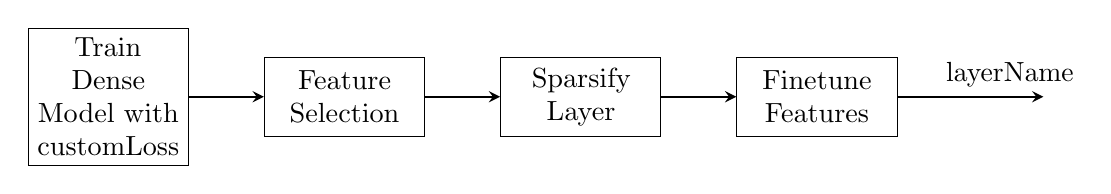
\begin{tikzpicture}[node distance=3cm]
\node (denseTraining) [process] {Train Dense Model with \gls{customLoss}};
\node (featureSel) [process, right of=denseTraining] {Feature Selection};
\node (fitSparse) [process, right of=featureSel] {Sparsify Layer};
\node (finetune) [process, right of=fitSparse] {Finetune Features};

\draw [arrow] (denseTraining) --   (featureSel);
\draw [arrow]  (featureSel) -- (fitSparse);
\draw [arrow] (fitSparse) --  (finetune);
\node(end) [right of=finetune] {};
\draw [arrow] (finetune) -- (end) node[midway, above, xshift=.5cm] {\gls{layerName}};
\end{tikzpicture}
    \caption{Overview of our proposed pipeline to construct a \gls{layerName}}
    \label{fig:OverviewAppraoch}
\end{figure*}
We propose a flexible, generally applicable method for generating a more locally and globally interpretable model with no need for additional labels and an adjustable tradeoff between interpretability and accuracy.
We make the decision process more interpretable by only using \gls{nReducedFeatures} features with  $\gls{nReducedFeatures} \ll \gls{nFeatures}$ and using an interpretable classifier \gls{classifyFunc}. At the core of an interpretable classifier \gls{classifyFunc} lies a linear layer $ \gls{outputVector} = \gls{WeightMatrix} \glsentrylong{featureVector} + \gls{bias}$
with the weight matrix \glsentrylong{WeightMatrix} and bias \glsentrylong{bias}. In order for it to be interpretable, \gls{WeightMatrix} has to be very sparse, meaning the number of non-zero entries  \gls{nWeights} has to be very low.~\citet{miller1956magical} showed that humans can handle $7\pm 2$ cognitive aspects at once, which constitutes an appropriate upper bound on the average number of relevant features per class $\gls{nperClass} = \frac{\gls{nWeights}}{\gls{nClasses}}$.
In our work we focus on $\gls{nperClass} \leq \tFs$.

The pipeline of our approach is presented in Figure~\ref{fig:OverviewAppraoch} and utilizes \glm{} for sparsification and feature selection.
We first train a deep neural network with our proposed feature diversity loss~\gls{customLoss} until convergence.
Then the features \Gls{trainFeatures} for all \gls{nTrainImages} images in the training set are computed,  which are the average pooled feature maps \Glspl{featureMaps}.
Afterwards, the features are selected as described in Section~\ref{sec:Selection} and \glm{}, presented in Section~\ref{sec:glmsaga}, is used to calculate the regularization path. 
Finally, the solution with the desired sparsity is selected from the regularization path and the remaining layers get finetuned with the final layer set to the sparse model, \st{} the features adapt to it.
\vspacehack{}
\subsubsection{Feature Diversity Loss}
\vspacehack{}
The goal of the proposed feature diversity loss \gls{customLoss} is that every feature captures a different independent concept. 
This is achieved by enforcing differently localized features in their feature maps.
The proposed loss is motivated by the \textit{Mutual-Channel Loss} (MCL)~\citep{DevilChannels} and the \textit{Feature Redundancy loss} (FRL)~\citep{ClassUniqueCorr}. In contrast to FRL, we use Cross-Channel-Max-Pooling (CCMP)~\citep{goodfellow2013maxout}  over all weighted feature maps to optimize all features jointly and reduce the need for the hyperparameter $K$. MCL also uses CCMP but instead of grouping the channels into class-specific filters, we apply the diversity component to all feature maps \Glspl{featureMaps}, to aim for shared interpretable features. For notation, $w_{\hat{c}l}$ describes the entry in \gls{WeightMatrix} that is assigned to the specific feature $l\in\displaystyle \{0, 1, \dots, \gls{nFeatures}-1 \}$ for the predicted class $\hat{c}= \arg\max(\gls{outputVector})\label{eq:MaxClassDiv}$ and $\gls{featureMaps}^l_{ij}=\Glspl{featureMaps}_{l,i,j}$.%
\begin{align}
\hat{s}^l_{ij} &=\frac{\exp(\gls{featureMaps}^l_{ij})}{\sum_{i'=1}^{\gls{featuresMapheigth}}\sum_{j'=1}^{\gls{featuresMapwidth}}\exp(\gls{featureMaps}^l_{i'j'})} \frac{\gls{featureVector}_l}{\max\glsentrylong{featureVector}}  \frac{|w_{\hat{c}l}|}{\Vert\boldsymbol{w}_{\hat{c}}\Vert_2} \label{eq:ScaleDiv}\\
     \gls{customLoss} &= -\sum_{i=1}^{\gls{featuresMapheigth}}\sum_{j=1}^{\gls{featuresMapwidth}}\max(\hat{s}^1_{ij},\hat{s}^2_{ij}, \dots, \hat{s}^{\gls{nFeatures}}_{ij})\label{eq:CCMPDiv}
\end{align}
Equation~\ref{eq:ScaleDiv} uses the softmax to transform the feature maps \Glspl{featureMaps} by normalizing their entries $\gls{featureMaps}^l_{ij}$ over the spatial dimensions and then %
scales the maps so that they focus on visible and important features by maintaining the relative mean of \Glspl{featureMaps} while weighting them according to the predicted class, \st{} different to MCL absent features do not have to be localized in small background patches.
Equation~\ref{eq:CCMPDiv} decreases the loss if the different weighted feature maps $\hat{S}^l$ attend to different locations.
The final training loss is then $\mathcal{L}_{\mathrm{final}} = \mathcal{L}_{CE} + \gls{cLW}\gls{customLoss}$
with the weighting factor $\gls{cLW}\in\mathbb{R}_+$.
\vspacehack{}
\subsubsection{Feature Selection}
\label{sec:Selection}
\vspacehack{}
For selecting the set of features \KeptFeatures{} from the initial features \initFeatures{} \st{} $\lvert\KeptFeatures\rvert=\gls{nReducedFeatures}$, we run an adapted version of \glm{}, introduced in Section~\ref{sec:glmsaga}, until one solution \psoln{j} of the regularization path  uses a feature not already in \KeptFeatures{}, which we then add to the set of selected features \KeptFeatures{} and restart the adapted \glm{}.
As adaptation, we extended the proximal operator of the group version of \glm{}, which operates on $\wl{l}=\gls{WeightMatrix}_{:,l}$, which are the entries in \gls{WeightMatrix} that correspond to an entire feature $l$. 
Since $\Vert\wl{l}\Vert_2$ indicates the importance of $l$, we additionally only keep entries for features that have the maximum norm or are in~\KeptFeatures{}, \st{} exactly one feature is added per iteration.
The resulting proximal operator with $\lambda_1 = \gamma\lambda\alpha$ and $\lambda_2 = \gamma\lambda(1-\alpha)$ is:
\begin{equation}
\textrm{Prox}_{\lambda_1, \lambda_2}(\wl{i}) = \begin{cases}
\frac{\wl{i}(\Vert\wl{i}\Vert_2 -\lambda_1)}{(1+\lambda_2)\Vert\wl{i}\Vert_2}
&\text{if }\Vert\wl{i}\Vert_2 > \lambda_1\underline{\land \Vert\wl{i}\Vert_2 = \max_{j'\in\initFeatures{}\setminus\KeptFeatures{}}\Vert\wl{j'}\Vert_2\lor i \in \KeptFeatures{}} \\
\boldsymbol{0} &\text{otherwise}
\end{cases}
\end{equation}
The extensions are underlined and  $\gamma$ is the learning rate of \glm{}.
\secondtablespot{}



\vspacehack{}
\section{Experiments}
\vspacehack{}
This section contains our experimental results. 
We validate our method using \gls{resNet}, \gls{denseNet} and \gls{incv}
on \fourtext{} common benchmark datasets in the domain of fine-grained image classification. Additionally, we show the applicability of a \gls{layerName} for large scale datasets like \glsentrylong{imgnetheader}.
An overview of \gls{cubheader}, \gls{stanfordheader}, \fgvcheader, \birdsheader{} and \imgnetheader{} is given in Table~\ref{table:DatasetOverview}.
 Additionally, \gls{cubheader} contains labels for the images such as attributes (\eg~“red wing”) as well as for the classes, which makes it easier to measure the alignment with understandable concepts.
 After the competitive accuracy and the impact of~\gls{customLoss} is shown, the interpretability of the \gls{layerName} is discussed and these attributes are used to show the alignment of the learned features.
The implementation details can be found in Appendix~\ref{app:ImpDetails}.
Finally, the tradeoff between interpretability and accuracy is visualized.

    
\firstTablespot{}








\subsection{Diversity Metric}
\vspacehack{}
To assess the impact of~\gls{customLoss}, we developed a measurement for the local diversity of the feature maps~\Glspl{featureMaps} that led to the decision, %
inspired by the diversity component of MCL~\citep{DevilChannels}, which entails a different way of computing the features. For that, we consider the $k$ feature maps $\Glspl{featureMaps}_k$ that are weighted the highest for the predicted class $\hat{c}$
in \gls{WeightMatrix}. 
To only compare the localization, softmax is applied to the $\Glspl{featureMaps}_k$, yielding $\boldsymbol{S}_k$.
With these distributions $\boldsymbol{S}_k$, we compute the diversity as%
\begin{equation}
    \loc{k} = \frac{\sum_{i=1}^{\gls{featuresMapheigth}}\sum_{j=1}^{\gls{featuresMapwidth}}\max(s^1_{ij},s^2_{ij}, \dots, s^k_{ij})}{k} 
\end{equation}
with $\loc{k}\in[\frac{1}{k}, 1]$ to measure
how different and pronounced
the $\Glspl{featureMaps}_k$ are localized. 
Since we focus on $\gls{nperClass} \leq 5$, we set $k=5$.
We report the mean \loc{5} for all classes that use at least \fivetext{} features.
Note that the proposed \gls{customLoss} is a weighted version of \loc{\gls{nFeatures}}.
\subsection{Results}
\label{sec:results}
\vspacehack{}
We report the accuracy on the test set for the dense model after training the pretrained model on the training data with $\gls{nperClass} = \gls{nFeatures}$, for the sparse model with $\gls{nperClass} \leq 5$, and for the result of our whole pipeline, the model with finetuned features, obtained by training the sparse model on the training data, and still $\gls{nperClass} \leq 5$.
Every shown metric is the average over \fivetext{} (\fourtext{} for \gls{imgnetheader}) randomly seeded runs. 
The standard deviations are included in the appendix.\\
Table~\ref{table:Accuracy incmp} shows 
the competitive performance of our \gls{layerName} to the dense \gls{resNet}.
It is evident that an extreme sparsity of $s = \frac{5}{2048}$
can be obtained in the final layer with just $0.1$ to $0.4$ percent points less accuracy. 
Additionally decreasing the number of features by $97.6\,\%$, resulting in just $50$ instead of the previous $2048$ features, only reduces the accuracy compared to the dense model by $1.3$ to $2.7$ percent points.
Finally, our proposed \gls{customLoss} improves the accuracy for all sparse models.
Table~\ref{table:Accuracy in backbone} shows the general applicability of our method with different backbones.
However, we observed some instability and no increased accuracy when finetuning the \gls{denseNet} with $\gls{nReducedFeatures}=2048$, showing a positive effect of sharing features. 
Table~\ref{tab:competitors} compares our approach to competitors: Without requiring additional supervision, we achieve a competitive performance compared to \glsentrylong{cbm}-based methods, while achieving a lower dimensionality and higher sparsity. Additionally, we improve the accuracy of \glm{} with heavily reduced \gls{nReducedFeatures}.
For \gls{imgnetheader}, we skipped the dense training and directly used the pretrained model.
The good scalability of our proposed method to this large dataset with a higher number of classes is displayed in Table~\ref{table:imgnetAccuracy}.
Table~\ref{table:loc5 in } shows the \loc{5}:
With \gls{customLoss} it is very close to the maximum value of $100\,\%$ in the dense case and still heavily increased in the sparse cases. This showcases that \gls{customLoss} is suitable to ensure a diverse localization and improved interpretability of the used feature maps
, which is visualized in Figures~\ref{app:fig:vizExamples0} to ~\ref{app:fig:vizExamples8}.
Finally, the total number of features that is used by the unrestricted ($\gls{nReducedFeatures} =\gls{nFeatures}$) models in Table~\ref{table:Accuracy incmp} is reduced from $912$ to $719$ for the models with~\gls{customLoss}, but still shows a high number of class-specific features.
That~\gls{customLoss} leads to more shared features supports our motivation of enforcing different features to capture different concepts.
\begin{table}
\resizebox{\linewidth}{!}{
\centering
\begin{tabular}{c|ccccc|ccccc|ccccc|ccccc}
\toprule
\fullheader 
\xmark & \textbf{\normalfont 86.6} & \normalfont 81.8 & \normalfont 85.3 & \normalfont 79.5 & \normalfont 83.4 & \normalfont 90.0 & \normalfont 88.4 & \normalfont 89.4 & \normalfont 87.3 & \normalfont 88.1 & \normalfont 84.2 & \normalfont 79.5 & \normalfont 83.3 & \normalfont 77.3 & \normalfont 80.7 & \normalfont 93.2 & \normalfont 90.9 & \normalfont 92.6 & \normalfont 89.3 & \normalfont 91.1 \\
\cmark & \textbf{\normalfont 86.6} & \textbf{84.0} & \textbf{86.5} & \textbf{81.7} & \textbf{84.0} & \textbf{91.4} & \textbf{90.7} & \textbf{91.1} & \textbf{89.8} & \textbf{90.1} & \textbf{84.4} & \textbf{81.0} & \textbf{84.0} & \textbf{79.8} & \textbf{81.7} & \textbf{93.6} & \textbf{92.1} & \textbf{93.3} & \textbf{91.1} & \textbf{92.0} \\
\bottomrule MCL~\cite{DevilChannels} & 86.1 & 81.9 & 85.1 & 79.4 & 82.8 & 90.1 & 88.4 & 89.0 & 87.2 & 88.1 &\emptyStrichte 93.1 & 91.0 & 92.5 & 89.0 & 90.7\\FRL~\cite{ClassUniqueCorr} & 86.4 & 81.5 & 85.3 & 78.9 & 82.6 & 90.0 & 88.5 & 89.4 & 87.5 & 88.2 &\emptyStrichte 93.3 & 90.8 & 92.6 & 89.4 & 90.9\\
\end{tabular}
}
\vspace{1mm}
\caption{Impact of the loss function on accuracy\inpercent{} for \resnet{}\bldStatement}
\label{table:Accuracy incmp}
\vspace{-5mm}
\end{table}



\begin{table}
\resizebox{\linewidth}{!}{
\centering
\begin{tabular}{c|ccccc|ccccc|ccccc|ccccc}
\toprule
\bbheader
\gls{denseNet} & 86.3 & \normalfont 76.2 & 82.9 & 75.7 & 83.1 & \textbf{91.5} & 88.2 & 89.8 & 88.1 & 90.0 & 84.1 & \normalfont 72.8 & \normalfont 64.6 & \normalfont 71.0 & 80.5 & 93.3 & \normalfont 87.3 & 91.7 & \normalfont 85.8 & 91.4 \\
\gls{incv} & \normalfont 82.3 & 78.0 & \normalfont 80.3 & \normalfont 74.0 & \normalfont 78.3 & \normalfont 88.9 & \normalfont 87.5 & \normalfont 88.1 & \normalfont 85.9 & \normalfont 87.4 & \normalfont 79.0 & 75.8 & 77.3 & 73.1 & \normalfont 76.5 & \normalfont 91.5 & 88.9 & \normalfont 90.3 & 86.3 & \normalfont 89.4 \\
\gls{resNet} & \textbf{86.6} & \textbf{84.0} & \textbf{86.5} & \textbf{81.7} & \textbf{84.0} & 91.4 & \textbf{90.7} & \textbf{91.1} & \textbf{89.8} & \textbf{90.1} & \textbf{84.4} & \textbf{81.0} & \textbf{84.0} & \textbf{79.8} & \textbf{81.7} & \textbf{93.6} & \textbf{92.1} & \textbf{93.3} & \textbf{91.1} & \textbf{92.0} \\
\bottomrule
\end{tabular}
}
\caption{Accuracy\inpercent{}\tablefinisher{backbone}\bldStatement}
\label{table:Accuracy in backbone}
\vspace{-.2cm}
\end{table}
\begin{table*}
\resizebox{\linewidth}{!}{
\centering
\begin{tabular}{ccc|cc}
\toprule
Dense ($\gls{nReducedFeatures}=2048$)  & Sparse ($\gls{nReducedFeatures}=2048$)  & Finet. ($\gls{nReducedFeatures}=2048$) & Sparse ($\gls{nReducedFeatures}=50$)  & Finet. ($\gls{nReducedFeatures}=50$) \\\midrule

76.1&\imgsunl&\imgfunl& \imgsl& \imgfl\\
\bottomrule
\end{tabular}
}
\caption{Accuracy\inpercent{}\imgbldStatement}
\label{table:imgnetAccuracy}
\vspace{-.3cm}
\end{table*}

\vspacehack{}
\subsubsection{Comparison with Other Loss Functions}
\vspacehack{}

\begin{table}
\resizebox{\linewidth}{!}{
\centering
\begin{tabular}{c|ccccc|ccccc|ccccc}
\toprule
\fullablheader
\xmark & \normalfont 50.2 & \normalfont 46.0 & \normalfont 43.4 & \normalfont 48.0 & \normalfont 46.5 & \normalfont 46.5 & \normalfont 43.8 & \normalfont 40.9 & \normalfont 45.9 & \normalfont 44.0 & \normalfont 45.0 & \normalfont 41.7 & \normalfont 39.1 & \normalfont 43.6 & \normalfont 43.7 \\
\cmark & \textbf{98.9} & \textbf{69.9} & \textbf{71.9} & \textbf{65.2} & \textbf{72.6} & \textbf{98.8} & \textbf{85.7} & \textbf{86.6} & \textbf{69.3} & \textbf{73.9} & \textbf{99.2} & \textbf{72.4} & \textbf{74.6} & \textbf{63.7} & \textbf{74.8} \\
\bottomrule MCL~\cite{DevilChannels} & 52.5 & 51.4 & 48.9 & 56.7 & 52.3 & 50.1 & 50.6 & 48.3 & 51.7 & 50.1 & 49.0 & 49.0 & 46.2 & 51.8 & 49.5\\FRL~\cite{ClassUniqueCorr} & 51.1 & 47.1 & 44.1 & 49.0 & 46.3 & 48.2 & 44.6 & 41.2 & 44.9 & 43.1 & 46.2 & 43.0 & 40.0 & 43.0 & 41.7\\
\end{tabular}
}
\caption{Impact of the loss function on \loc{5}\inpercent{} for \resnet{}\bldStatement}
\label{table:loc5 in }
\vspace{-.3cm}
\end{table}







We compare our diversity loss \gls{customLoss} with the MCL~\citep{DevilChannels} and the FRL~\citep{ClassUniqueCorr}. 
The used hyperparameters for the loss functions are reported in Appendix~\ref{app:cbmjoint} and we focussed on three datasets to save computational resources.
Table~\ref{table:Accuracy incmp} shows that our \gls{customLoss} reaches the highest accuracy across all datasets. Notably, the accuracy reported in~\citep{DevilChannels} for the MC-Loss is achieved by a two-layer MLP plus additional techniques, whereas we only use one layer to ensure linearly separable representations for our \gls{layerName}. %
Although it is expected that applying \gls{customLoss} has a positive effect on \loc{5} due to the similar formulation, we could observe a remarkable uplift in \loc{5} (Table~\ref{table:loc5 in }) compared to MCL and FRL, which also optimize for differently localized features.














\subsection{Interpretability}%
\label{Exp:Interpretability}
\vspacehack{}
\begin{figure*}     
        \vspace{-0.45cm}
     \begin{subfigure}[t]{.47\textwidth}
         \centering
            \includegraphics[width=\textwidth]{plots/AssignedClasses.png}
        \caption{Exemplary \sparsemat. The alignment of the features with attributes in CUB-2011 is displayed in Figure~\ref{fig:AttMatrix}.}
        \label{fig:Matrix}
     \end{subfigure}
     \hfill
     \begin{subfigure}[t]{.47\textwidth}
         \centering
       \includegraphics[width=\textwidth]{plots/Th0.2Sorted_1_AssignedFeatures14.png}
            \caption{Relationship between chosen features and attributes ($C > 20\%)$ of CUB-2011 for the exemplary model. Higher values indicate that the feature describes the attribute.  }
        
\label{fig:AttMatrix}
     \end{subfigure}
     \caption{Visualization of the sparse matrix and the feature alignment.}
        \label{fig:matrices}
\end{figure*}
In this section, we discuss the interpretability of the proposed \gls{layerName} using example models.
The interpretability of the proposed \gls{layerName} is based upon using very few (\gls{nperClass}) features from a small pool of \gls{nReducedFeatures} to make a decision. A low \gls{nReducedFeatures} allows the analysis of the remaining features to try to align them with a human understandable concept, which is discussed in Section~\ref{sec:AlignmentFeatures}.
Since the sparse linear layer is easily interpretable%
, the complete model with sufficiently well understood features is both \textbf{locally} and \textbf{globally} interpretable.\\
For \textbf{global interpretability}, the 
final layer of the \gls{layerName} 
can be fully visualized and analyzed. Figure~\ref{fig:Matrix} shows $\gls{WeightMatrix}^{\mathrm{sparse}}$.
This allows the practitioner to verify the global behavior of the model.
For example, the attribute aligned with \enquote{has-bill-shape:needle} in the presented model in Section~\ref{sec:AlignmentFeatures} has a non-zero weight for all \fourtext{} classes that have the attribute in more than 30\,\% of examples. 
The visualization of the classes positively related to a specific attribute and features related to a class like Figures~\ref{app:fig:vizExamples0} to ~\ref{app:fig:vizExamples8} helps to trust the model.
Additionally, $\gls{WeightMatrix}^{\mathrm{sparse}}$ allows for further feature understanding, since it is possible to analyze the similarities between classes that share a feature. %
If the feature is aligned well, this leads to knowledge discovery.\\  
The \textbf{local interpretability} describes the explanation of a single decision made by the model. Decisions with sparsely connected features are inherently locally interpretable, if the features can be interpreted and localized, as shown in Figure~\ref{fig:Cover}. 
The practitioner can understand where and what was found in the image, and due to the full global interpretability also understand the behavior around the current example.

\vspacehack{}
\subsubsection{Feature Alignment}
\label{sec:AlignmentFeatures}
\vspacehack{}
In this section, we demonstrate how the features of the proposed \gls{layerName} can be aligned with interpretable concepts.%
We describe how one can use additional labels or expert knowledge to interpret the features and demonstrate that several learned sparse features are directly connected to attributes relevant to humans. Thus, our model learns such abstract concepts directly from the data.
Overall, due to the very limited number of used features \gls{nReducedFeatures}, the features can and should be thoroughly analyzed and interpreted to facilitate interpretability.
For feature localization, we follow a masking approach similar to~\citet{fong2017interpretable}, which is described in Appendix~\ref{app:featureViz}.
\paragraph{Alignment with Additional Data}
\begin{figure*}
     \begin{subfigure}[t]{.47\textwidth}
         \centering
         \includegraphics[width=\textwidth]{plots/SchnabelVizScaledPfeilGrad.png}
         \caption{Feature $45$ with $C=0.39$ for the attribute \enquote{has-bill-shape:needle}: Higher activations are localized around the bill, and a needle-like bill is visible. }
         \label{fig:Schnabel}
     \end{subfigure}
     \hfill
     \begin{subfigure}[t]{.47\textwidth}
         \centering
       \includegraphics[width=\textwidth]{plots/2StrahligFlugzeugScaled.png}
         \caption{Manually aligned feature of a model trained on FGVC-Aircraft without additional labels: The feature is manually aligned with four engine aircraft as shown in Appendix~\ref{app:sec:alignment}.}
         \label{fig:4Strahlig}
     \end{subfigure}
        \caption{Example images and localization \gls{LocalizationMaps}, scaled to indicate feature activation, in ascending order for two models. The text between the rows describes the activation value for the image, which drops below 0 due to the normalization of \glm{}, and the class name. }
        \label{fig:three graphs}
        \vspace{-0.35cm}
\end{figure*}

We use the attributes $A$ contained in CUB-2011 to align the learned features with these labels after the finetuning. 
For each attribute $a \in A$ and feature $j$ we compute a score $C_{aj}$ that corresponds to a relative increase of the feature when the attribute is present:
\begin{align}
\delta_{aj} = \frac{1}{\lvert\attributeset{a+}\rvert}\sum_{i\in\attributeset{a+}}\gls{trainFeatures}_{i,j}- \frac{1}{\lvert\attributeset{a-}\rvert}\sum_{i\in\attributeset{a-}}\gls{trainFeatures}_{i,j} &&
    C_{aj} = \frac{\delta_{aj}}{\max(\gls{trainFeatures}_{:,j}) - \min(\gls{trainFeatures}_{:,j})} 
\end{align}
The set of indices whose images contain the attribute is denoted by~\attributeset{a+}.
We considered an attribute to be present if the human annotated it with \enquote{probably} or \enquote{definitely}.  Annotations with \enquote{guessing} were neither included in the positive (\attributeset{a+}) nor negative (\attributeset{a-}) examples.
For one exemplary model a part of the matrix of $C$ values is displayed in Figure~\ref{fig:AttMatrix}. 
It is clear, that some features correspond to colors, some to specific shapes like “bill-shape:needle” and other features do not correlate with specific attributes. 
Figure~\ref{fig:Schnabel} visually validates the connection that was implied in Figure~\ref{fig:AttMatrix}.
\paragraph{Manual Alignment}
To ensure that the entirety of a feature is understood, or in absence of additional data, the features have to be manually aligned for increased interpretability. This is enabled by the low number of features and sparsity.
Some useful aspects for understanding a feature are the localization, extreme examples, feature visualization~\citep{olah2017feature} or which classes use that feature. One such alignment for a model trained on FGVC-Aircraft is displayed in Appendix~\ref{app:sec:alignment} and Figure~\ref{fig:4Strahlig}.
Aligning learned features with human understandable concepts is still challenging as a single feature can refer to multiple aspects and human understandable concepts do not need to be axis aligned~\citep{szegedy2013intriguing}. However, the low dimensionality of the remaining features allows for a sophisticated analysis of every feature in practice, which could even discover spurious correlations as features as done by the \glm{} publication.
\subsection{Interpretability Tradeoff}
\vspacehack{}


\begin{figure}
\centering
\hspace{0.05\linewidth}
     \begin{subfigure}[t]{.4\linewidth}
         \centering
         \includegraphics[width=\textwidth]{plots/nfeatures.png}
          
         \caption{Impact of changing \gls{nReducedFeatures} with $\gls{nperClass}=5$ }
         \label{fig:NFeaturesImpact}
     \end{subfigure}
     \hfill
     \begin{subfigure}[t]{.4\linewidth}
         \centering
         
       \includegraphics[width=\textwidth]{plots/nWeights.png}
       
         \caption{Impact of changing \gls{nperClass} with $\gls{nReducedFeatures}=50$ or $2048$ }
         \label{fig:Impactnwc}
         
     \end{subfigure}
     \hspace{0.05\linewidth}
        \caption{Relationship between Finetune Accuracy and aspects related to interpretability for \gls{resNet}. }
        \label{fig:ContinousInt}
    \vspace{-.2cm}
\end{figure}

In this section, we analyze the impact of changing \gls{nReducedFeatures} and \gls{nperClass} on the finetuning accuracy of the model trained with \gls{customLoss}, shown in Figure~\ref{fig:ContinousInt}. 
Figure~\ref{fig:NFeaturesImpact} visualizes the impact of \gls{nReducedFeatures}: 
With decreasing \gls{nReducedFeatures} the accuracy drops slowly until a dataset-specific threshold is reached, at which a steep decline starts.
Additionally, the proposed~\gls{customLoss} works regardless of~\gls{nReducedFeatures}. 
Figure~\ref{fig:Impactnwc} shows the finetuning accuracy in relation to \gls{nperClass}: 
The accuracy is rather insensitive to \gls{nperClass},
only decreasing when $\gls{nperClass}<5$, which is the case for both dimensions and showcases that \fivetext{} features suffice for a competitive model even if the features are shared among classes.
Figure~\ref{fig:ContinousInt} demonstrates the tradeoff that our \gls{layerName} offers: Both \gls{nperClass} and \gls{nReducedFeatures} can be drastically reduced with either a negligible or small impact on accuracy to adapt to the amount of interpretability needed.


























\vspacehack{}
\section{Limitations and Future Work}
\label{sec:limits}
\vspacehack{}
As shown in Figure~\ref{fig:ContinousInt}, the \gls{layerName} cannot get arbitrarily low-dimensional or sparse with competitive accuracy via our proposed method. 
The optimal sparsity and dimensionality for a given problem are hard to predict and might require some experiments to determine the minimum values for competitive accuracy.
Aligning all used features with human concepts is still difficult, albeit more feasible than without a \gls{layerName}.
Future work could use a more interpretable feature extractor like \textit{B-cos Networks}~\citep{bohle2022b} to alleviate that problem.
\reinderscite{}
It seems promising to apply a \gls{layerName} to other safety-critical domains, such as medical, where an expert can be utilized to align the features and follow the decision, as it can help bring the required interpretability and trustworthiness to the domain.
Embodied autonomous agents can also benefit from it, as the entire decision process can be thoroughly analyzed.
\rudolphcite{}
While more interpretable models could be used to more deliberately bring harm, they can disclose existing problems with machine learning models and open up the opportunity to build fair and trustworthy models.
Finally, sparsity and dimensionality could be part of metrics used to quantify the trustworthiness of a model.
\section{Conclusion}
\vspacehack{}
In this work, we proposed the more interpretable sparse low-dimensional decision model (\gls{layerName})  to allow a human to follow and understand the decision of a Deep Neural Network for image classification.
Our proposed pipeline constructs a \gls{layerName} with drastically increased global and local interpretability while still showing competitive accuracy.
As demonstrated, a practitioner can manually configure the pipeline to set the tradeoff between accuracy and interpretability.
Our novel loss increases the feature diversity and we showed that identifying a class with varied features can improve the accuracy. 
Finally, our \gls{layerName} offers measurable aspects of interpretability, which allows future work to not just compare itself on accuracy but also on interpretability.
















